\chapter{Results} % Main appendix title

\label{AppendixD} % For referencing this appendix elsewhere, use \ref{AppendixX}

\section{Ford AV Dataset steering angles}

\subsection{Ford AV Dataset}

The steering angles can be extracted from .bag files using ROS commands:
\begin{verbatim}
    # In one terminal, start ros engine
    $ roscore
    # In another terminal, inspect content of bag file
    $ time rosbag info Sample-Data.bag
    (...)
             /imu                 146939 msgs    : sensor_msgs/Imu             
    (...)
             /pose_ground_truth   146136 msgs    : geometry_msgs/PoseStamped   
             /pose_localized       16100 msgs    : geometry_msgs/PoseStamped   
             /pose_raw            146190 msgs    : geometry_msgs/PoseStamped   
(...)
    # And subscribe to topic of interest 
    $ rostopic echo /imu | tee sample_imu.yaml
    # In another terminal, playback bag file
    $ time rosbag play --immediate Sample-Data.bag --topics /imu
    # Sanity check, count number of acquisitions
    $ cat sample_imu.yaml | grep "orientation:" | wc -l
\end{verbatim}
The snippet above generates file imu.yaml, with all pose data generated by imu device. From this file we extract the steering angle, which is the z axis (yaw) of the orientation field (TODO check .yaml dialect). 
Images can be extracted from the same bag file with the Python 2.7 bag\_to\_images.py script:
\begin{verbatim}
    $ python2 bag_to_images.py Sample-Data.bag ~/git/msc-data/ford/sample/ros/ \
        /image_front_left
\end{verbatim}
Each image is an attribute in a dictionary, which also contains seconds (secs) and nano seconds (nsecs) attributes within the header attribute:
\begin{verbatim}
header: 
  seq: 213414
  stamp: 
    secs: 1501822147
    nsecs: 684951066
  frame_id: "camera_front_left"
height: 215
width: 414
encoding: "8UC3"
is_bigendian: 0
(...)
\end{verbatim}
Thus a timestamp can be obtained for each image extracted. This is done with script parse\_yaml\_time.py:
\begin{verbatim}
    
\end{verbatim}
While the steering angles are extracted 
The image can be matched with a steering angle by obtaining the timestamp of image, the full secs 

\section{Audi}

The  Audi Autonomous Driving Dataset (A2D2)
authors (\cite{geyer2020a2d2}) are motivated by the fact that research in machine learning, mobile robotics and autonomous driving is accelerated by the availability of high quality annotated data. This statement can be verified by the advances in image classification with deep neural networks since \cite{IMAGENET} became available.  
The A2D2 data was acquired with a human-driven Audi Q7 e-tron equipped with six cameras (front left, front center, front right, back left, back center, back right) and five LiDAR sensors. The authors claim this resulted in  360$^{\circ}$ camera and LiDAR coverage. Additionally, several bus data signals from the vehicle were recorded such as velocity, acceleration and steering wheel angle. 
The total size is 2.3TB. Our datasets of interest are the  Though, since we are interested in image and steering angle only, our data can be narrowed to 
\begin{verbatim}
    https://aev-autonomous-driving-dataset.s3.eu-central-1.amazonaws.com/README-SensorFusion.txt
    
- steering_angle_calculated
- steering_angle_calculated_sign

- 'cam_front_center'
\end{verbatim}

The dataset total size is approximately 2.3TB and provides (...) TBC following https://www.a2d2.audi/a2d2/en/download.html

This was supplied for three cities: Gaimersheim, Ingolstadt and Munich. To perform initial investigations we chose data from Munich and downloaded the "Camera - Front Center" images, constituting 27451 images 3.2MB in size each and dimension 1920x1208 pixels, total size on disk is about 92GB. We also downloaded the 176MB "Bus Signals" file. The image naming convention uses a timestamp in the format:
\begin{verbatim}
20190401145936_camera_frontcenter_000017970.png
\end{verbatim}
The "Bus Signals" file is JSON encoded and provides several signals such as acceleration, angular velocity and vehicle speed. Our signals of interest are the steering angle calculated and steering angle sign. In the bus signals file (20190401121727\_bus\_signals.json) we parsed our values of interest e.g.
\begin{verbatim}
(...)
    "steering_angle_calculated": {
        "unit": "Unit_DegreOfArc",
        "values": [
            [
                1554115464698116,
                2.4
            ],
(...)
\end{verbatim}
where the unit is degree of arc and the values are inferred to be a timestamp when the measurement was acquired and the angle (1554115464698116 and 2.4 respectively, in the example shown).
and found 91968 entries for each of the steering angle and sign. This is over 3 times the amount of corresponding images. Since there was no obvious key to match the steering angle and sign with a corresponding image, we wrote to the supplied enquiry email address aevdrivingdataset@audi.de with regard to this problem and receiving no reply, abandoned the dataset deeming it unusable for our purposes.  
Note: we did try converting the integer into a date using python, which resulted in an error:
\begin{verbatim}
import datetime
audi_timestamp = 1554115464698116
date = datetime.datetime.fromtimestamp(audi_timestamp / 1e3)
print(date)
# ValueError: year 51217 is out of range    
\end{verbatim}

%% TODO add correspondence with Mentar

\section{Unity3D changing sky hue}
The simulator is started by running:
\begin{verbatim}
$ sudo ~/.Unity.AppImage --no-sandbag   
\end{verbatim}
This will load the Unity Hub application. A project can be added, which will be repository cloned from \cite{SDSandboxSim}. Once loaded, the menu scene is selected and the project is run. Once running, an output directory must be chosen. A track is then selected (TODO track list), then the option "Auto with REC TODO double check".  
TODO ADD IMAGE SEQUENCE  
Once a number of laps have been completed, the images can be moved to a labelled folder using prepare\_data.py script. This will move images to a user defined directory, create a sub-directory named with a date and timestamp

The sky colour can be changed via Windows > Renderer > Lighting menu, then under Environment changing "Skybox Material".

Changing camera sensor image output size

There are two ways to change the size of images output by simulator camera sensor, one is by editing Donkey.Prefab file and changing lines 3415 and 3416:
\begin{verbatim}
  width: 160
  height: 120
\end{verbatim}
The other was is through Unity
Changing sky colour
The sky colour can be changed via Windows > Renderer > Lighting Settings menu, then under Environment changing "Skybox Material" chossing a different material.  
The simulator lighting can be made darker, in the same menu, under Environment Lighting > Intensity MUltiplier. A value of 1 is chosen to generate training datasets, and a value of 0.26 when running the simulator in NN Control over Network mode, that is using the prediction engine to predict steering angles.
\section{Udacity}

1. Link trail - medium (Indian guy) -> medium (Chinese guy)-> github (Japanese guy)  
  
2. Udacity data  
Data is available for download in torrent file format (\cite{torrentCite}) and consist of Robot Operating System (ROS) rosbag compressed files.

\begin{verbatim}
https://github.com/udacity/self-driving-car/tree/master/datasets
\end{verbatim}
3. Rosbag

\section{utbm}
More stuff from german uni?
\begin{verbatim}
https://epan-utbm.github.io/utbm_robocar_dataset/
\end{verbatim}

TODO ADD BINS
\begin{figure}[ht]
 \centering 
 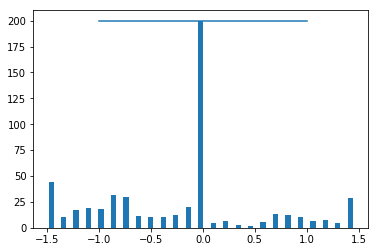
\includegraphics[scale=1]{Figures/bins.png}
 \caption{Diagram showing bins centered around zero degrees, meaning most of time car is driving straight. Binning diagrams for all datasets can be found in appendix B}
 \label{fig:bins-placeholder}
\end{figure}

\section{Training Log}

\begin{verbatim}
Run ID  Data       Network Acc. Error Saved Best Model 
3       log_sample NVIDIA1
\end{verbatim}

Run ID  Data    Network Training    Acc Error   Saved Best Model    Saved History
%1       Udacity 1       SGD Adam    .95 .06     model_01            history_01

\subsection{Run 3}

This model has a single output, steering angle, and produced very low accuracy.
Notes:
\begin{verbatim}
commit 423b5b783565b60e72f970485d9b3aa9887f5453
training time
dataset: sample_data
\end{verbatim}

\subsection{Run 4 - }

% Naoki's model not doing well, sanity check with one output
Also not doing well
Next run, 2 outputs (steering and throttle)

\subsection{Run 5 - 20201102081239} 

\begin{verbatim}
commit 076e8b32664738df6af9e14d75355504eb2a94b4
Much better results with two outputs. 
cat ../dataset/unity/log_sample/logs_Mon_Jul_13_08_29_01_2020/record_11659.json
Both are floats - steering angle and throttle
loss: 0.0105 - acc: 0.8502 - val_loss: 0.0111 - val_acc: 0.8617

dataset: sample_data
model: nvidia1
outputs: 2

Comment: Network trained with no augmentation of cropping.

\end{verbatim}

From this point onwards, a model name, if generated, is given with every run.

\subsection{Run 5 - 20201102090041\_nvidia2}
\begin{verbatim}
commit 42dabb6321ad25f667c8663b63412c88c96b3b38
model: nvidia2
outputs: 2
dataset: log_sample (size: 12k)
$ python train.py --model=nvidia2 --outdir=../trained_models
loss: 0.0108 - acc: 0.8483 - val_loss: 0.0117 - val_acc: 0.8495
\end{verbatim}

\subsection{Run 6 - 20201102094552\_nvidia1}
\begin{verbatim}
commit ec9d081b85f7386365428a73896b1d09be7ba917
model: nvidia1
outputs: 2
dataset: genRoad (280727)
command
$ train.py --model=nvidia1 --outdir=../trained_models
loss: 0.0077 - acc: 0.8726 - val_loss: 0.0077 - val_acc: 0.8732

Comment: Network trained with no augmentation of cropping.

video upload: https://youtu.be/ZLhrcyuONj0
\end{verbatim}

\subsection{Run 7 - 20201102090041\_nvidia2.h5}
\begin{verbatim}
commit 1da10b6745f583e180d5b9c5ba4874847ba8610c
model: nvidia2
outputs: 2
Dataset: genRoad
command
$ train.py --model=nvidia2 --outdir=../trained_models
\end{verbatim}

\subsection{Run 8 - 20201102134802\_nvidia2.h5}
\begin{verbatim}
commit 6960f2f5fb50b565c0dfd6c8fe3ac1d283192e69
model nvidia2
outputs 2
dataset log2
command:
train.py --model=nvidia2 --outdir=../trained_models
\end{verbatim}


\subsection{Run 9 - 20201102210514\_nvidia2.h5}
\begin{verbatim}
Running nvidia2 with augmentation
commit 6960f2f5fb50b565c0dfd6c8fe3ac1d283192e69
model nvidia2
outputs 2
dataset log2
command:
train.py --model=nvidia2 --outdir=../trained_models
loss: 0.0345 - acc: 0.7906 - val_loss: 0.0236 - val_acc: 0.8084
Stop! Still running!!! Epoch 60 and still improving. ...
% loss: 0.0193 - acc: 0.8250 - val_loss: 0.0116 - val_acc: 0.8503
% 0.0123 - acc: 0.8501 - val_loss: 0.0091 - val_acc: 0.8594
Ran 78 epochs and may have thrown error:
problems with loss graph
Note biggest increase in accuracy during training
\end{verbatim}

\subsection{Run 10 - 20201103211330\_nvidia2.h5}
\begin{verbatim}
Run nvidia2 WITHOUT augmentation, just preprocessing
commit 2add77bb60505fe25075f9da55f6465e65cd3825
model nvidia 2
outputs 2
dataset log2
command:
train.py --model=nvidia2 --outdir=../trained_models
loss: 0.0233 - acc: 0.8179 - val_loss: 0.0170 - val_acc: 0.8304
loss: 0.0084 - acc: 0.8656 - val_loss: 0.0086 - val_acc: 0.8655
Epoch 45/100
loss: 0.0083 - acc: 0.8662 - val_loss: 0.0086 - val_acc: 0.8638
problems with loss graph

No loss graph, again, no augmentation trained quicker that previous

\end{verbatim}

\subsection{Run 11}
\begin{verbatim}
commit 6439a8758d8b46a1cbc3bcefc9db4c15f70820df
model nvidia1
outputs 2
dataset log 2
command:
train.py --model=nvidia1 --outdir=../trained_models
Epoch 1/100
1755/1755 [==============================] - 682s 389ms/step - loss: 0.0271 - acc: 0.8049 - val_loss: 0.0172 - val_acc: 0.8351
Epoch 84/100
1755/1755 [==============================] - 559s 318ms/step - loss: 0.0099 - acc: 0.8581 - val_loss: 0.0083 - val_acc: 0.8662
problems with loss graph (probably a bug introduced in adding info to graph?)

\end{verbatim}

\subsection{Run 12}
\begin{verbatim}
commit augment.ipynb
model nvidia_baseline
outputs 1
dataset log2 (280746)
command:
train.py --model=nvidia_baseline --outdir=../trained_models

There is an issue with the aspect ratio and cropping, need to investigate with augment.ipynb

Note log2 was renamed genRoad as it is exactly that and a more descriptive name.
ls
\end{verbatim}

\subsection{Run 13}
\begin{verbatim}
commit e14e4bb9bdd0d322867c6cdba706478f662e71f6
model nvidia_baseline
outputs 1
dataset log (45421)cd 
command:
train.py --model=nvidia_baseline
--outdir=../trained_models
--epochs=1
--inputs=../dataset/unity/log/*.jpg
--aug=True
--preproc=True

Comment: ran ok for one epoch, images sized correctly.
Adding more epochs
\end{verbatim}

\subsection{Run 14}
\begin{verbatim}
commit e14e4bb9bdd0d322867c6cdba706478f662e71f6
model nvidia_baseline
outputs 1
dataset log
command:
train.py --model=nvidia_baseline
--outdir=../trained_models
--epochs=100
--inputs=../dataset/unity/log/*.jpg
--aug=True
--preproc=True

Comment: Started with very low accuracy.
Stopped process as error seems to have gone out of range
Epoch 5/100
283/283 [==============================] 
- 107s 377ms/step - loss: nan - acc: 5.5259e-05 
- val_loss: nan - val_acc: 1.1004e-04
\end{verbatim}

\subsection{Run 15}
\begin{verbatim}
commit aec3290fdbc83e71e450deef650aa2d51873b886
model nvidia_baseline
outputs 2
dataset log
command:
train.py --model=nvidia_baseline
--outdir=../trained_models
--epochs=100
--inputs=../dataset/unity/log/*.jpg
--aug=True
--preproc=True
Comment: Started at loss: nan - acc: 0.4305. Two outputs definitely helps. Why?
Perhaps because model is not going around track at constant speed?

\end{verbatim}

\subsection{Run 16}

\begin{verbatim}
commit 10a3fc2f6d23e04f604914c1f8420e574a8ce808
model nvidia_baseline
outputs 2
dataset log
command:
train.py --model=nvidia_baseline
--outdir=../trained_models
--epochs=100
--inputs=../dataset/unity/log/*.jpg
--aug=True
--preproc=True
Comment: Added linear activation in final layer, loss returning a reasonable value:
loss: 1.2035 - acc: 0.5404
Turned into nan on 3rd epoch. Accuracy going down, stopping process
\end{verbatim}

\subsection{Run 17}

\begin{verbatim}
Commit: a76169106a9087f5cc7e851fe09294699bb6240c 
Model: nvidia_baseline
Outputs: 2
Dataset: genRoad
Command: 
train.py --model=nvidia_baseline
--outdir=../trained_models
--epochs=100
--inputs=../dataset/unity/log/*.jpg
--aug=True
--preproc=True

Comment: Removed weight decay
Still loss taking NaN values
Epoch 13/100
281/281 (...) val_loss: nan - val_acc: 0.4939

\end{verbatim}

\subsection{Run 18 }

\begin{verbatim}
Commit: baa8f3d066dc37d3c2bb7792fa9db4801824d1bb 
Model: nvidia_baseline
Outputs: 2
Dataset: genRoad
Command: 
train.py --model=nvidia_baseline
--outdir=../trained_models
--epochs=100
--inputs=../dataset/unity/log/*.jpg
--aug=True
--preproc=True
Comment: Removed dropout from last dense layer. Training loss NaN on first epoch.
Dropout added again, loss back to under 1. Seems to have an influence, trying
multiple dropout removals next.

\end{verbatim}



\subsection{Run 19}
\begin{verbatim}
Commit: 16a6f8ffc6399143e7ad5a6885ee9b44b3ca1dda
Model: nvidia_baseline
Outputs: 2
Dataset: genRoad
Command: 
train.py --model=nvidia_baseline
--outdir=../trained_models
--epochs=100
--inputs=../dataset/unity/log/*.jpg
--aug=True
--preproc=True
Comment: Left one dropout (.25) layer, loss still NaN.
\end{verbatim}

\subsection{Run 20}

\begin{verbatim}
Commit: d7e05ad1cdf0fab3a83975be259feb16830b5a38
Rest same as 19
Comment: Removed Dense(1164) layer. Loss is Nan on first epoch.
Stopping run

\end{verbatim}

\subsection{Run 21}
\begin{verbatim}
Commit: d8fb9705dd676554dcf84a213b3c27d0e1f9d0c4 
Rest same as 19
Comment: Loss is Nan on first epoch
Epoch 1/100
(...)loss: nan - acc: 0.5017
\end{verbatim}

\subsection{Run 22}
\begin{verbatim}
Commit: ba4432568a589eac5a7d7c4927fa96e2f9e11bd1
Model, Outputs, Dataset and Command: Same as 19
Comment: Using Glorot Uniform (Xavier) kernel initializer.
Loss in Nan on first epoch. Training stopped.
Epoch 1/100
284/284 [==============================] - 101s 357ms/step - loss: nan - acc: 0.4609
\end{verbatim}

\subsection{Run 23}
\begin{verbatim}
Commit: 5cba2c7b01a160e7053e09220e63b1c575cf51e8  
Model, Outputs, Dataset and Command: Same as 19
Comment: All biases initialized to 0.
Loss in Nan on first epoch. Training stopped.
Epoch 1/100
283/283 (...) loss: nan 
\end{verbatim}

\subsection{Run 24}
\begin{verbatim}
Commit: 56aea3e16bb0f9db5735dfa536809389f35b12da  
Model, Outputs, Dataset and Command: Same as 19
Comment: Removed Dense(10) layer
Loss in Nan on first epoch. Training stopped.
\end{verbatim}

\subsection{Run 25}
\begin{verbatim}
Commit: 6a8ee72727db2508d2ff1ae35d068837a5b524ab  
Model, Outputs, Dataset and Command: Same as 19
Comment: Increased dropout to 0.5.
Loss in Nan on second epoch. Training stopped.
Epoch 1/100
285/285 [==============================] - 100s 352ms/step 
- loss: 0.0660 - acc: 0.6910 - val_loss: 0.0299 - val_acc: 0.7809
Epoch 2/100
285/285 [==============================] - 100s 350ms/step - loss: nan - acc: 0.5000
\end{verbatim}

\subsection{Run 26}
\begin{verbatim}
Commit: e4a287dc816a2a4d2c47893b131c710b2ecb8594  
Model, Outputs, Dataset and Command: Same as 19
Comment: Spreading 0.5 dropout between layers (0.1 each).
Loss in Nan on third epoch. Training stopped.
Epoch 3/100
284/284 (...) loss: nan
\end{verbatim}

\subsection{Run 26}
\begin{verbatim}
Commit: 2e5bf1b7002a2ddbbe2fea003fce010627d723e2  
Model, Outputs, Dataset and Command: Same as 19
Comment: Changed layer dropout to 0.15.
Loss in Nan on first epoch. Training stopped.
\end{verbatim}

\subsection{Run 27}
\begin{verbatim}
Commit:   
Model, Outputs, Dataset and Command: Same as 19
Comment: Changed layer dropout to 0.05.
Loss in Nan on first epoch. Training stopped.
\end{verbatim}

\subsection{Run 28}
\begin{verbatim}
Commit: 9a70ff7e194736a475bdce0b6eddc65aad6ea8c0  
Model, Outputs, Dataset and Command: Same as 19
Comment: Changed number of kernels on 2nd Conv layer to 32.
Loss in Nan on first epoch. Training stopped.
\end{verbatim}

\subsection{Run 29}
\begin{verbatim}
Commit:   
Model, Outputs, Dataset and Command: Same as 19
Comment: Changed number of kernels on 3nd Conv layer to 64.
Loss in Nan on first epoch. Training stopped.
\end{verbatim}

\subsection{Run 30}
\begin{verbatim}
Commit: 1997b914e829466659a27bfe1b31a6a6374afd36  
Model, Outputs, Dataset and Command: Same as 19
Comment: Changed aspect ratio to 160x120
Loss in Nan on 2nd epoch. Training stopped.
Epoch 2/100
283/283 (...) loss: nan - acc: 0.5982
\end{verbatim}

\subsection{Run 31}
\begin{verbatim}
Commit: 1997b914e829466659a27bfe1b31a6a6374afd36  
Model, Outputs, Dataset and Command: Same as 19
Comment: Changed aspect ratio to 160x120
Loss in Nan on 2nd epoch. Training stopped.
Epoch 2/100
283/283 (...) loss: nan - acc: 0.5982
\end{verbatim}

\subsection{Run 32 - 20201117154210\_nvidia\_baseline.h5}
\begin{verbatim}
Commit: 1997b914e829466659a27bfe1b31a6a6374afd36  
Model: nvidia_baseline
Outputs: 2
Dataset: smallLoopingCourse (jungle1) (34443)
Command: 
train.py --model=nvidia_baseline
--outdir=../trained_models
--epochs=100
--inputs=../dataset/unity/genTrack/log/*.jpg
--aug=True
--preproc=True
Comment: Loss in Nan on 1st epoch. Training stopped.
This run also produced a usable model.
\end{verbatim}

\subsection{Run 33}
\begin{verbatim}
Commit: 861095ac1a997e0f460aca6ceda93df98b7d0a48  
Model, Outputs, Dataset and Command: Same as 19
Comment: Explicitly setting strides=(1,1) is conv layers 4 and 5.
Loss in Nan on 1st epoch. Training stopped.
\end{verbatim}

\subsection{Run 34 - 20201117162326\_nvidia\_baseline.h5}
\begin{verbatim}
Commit: d0b7160793ee433ed25724d966a7d3bd85ae8ffa  
Model, Outputs, Dataset and Command: Same as 19
Comment: Changed batch size to 64
Loss is NaN on 7th epoch
Epoch 7/100
567/567 (...) loss: nan

This run produced a usable model.
\end{verbatim}

This run consisted of a sanity check to determine if training would generate a loss value different from NaN (not a number). This was not the case as per results in comments.

\subsection{35 - 20201120124421\_nvidia\_baseline.h5}
\begin{verbatim}
Commit: 1f5c64bc219b31cf8654d2cceec910f0dea5ecbf
Model: nvidia_baseline
Outputs: 2
Dataset: log_sample (12894 - small looping track)
Environment: simbox (local)
Command: 
--model=nvidia_baseline --outdir=../trained_models --epochs=100 --inputs=../dataset/unity/log_sample/*.jpg --aug=True --preproc=True

Comment: Sanity check run, with the aim of
establishing a repeatable training session, aiming
at debbugging Keras when the need arises, that is
when Keras is suspected of somehow having become 
corrupted. 

Note before running, all .jpg images were found to have corresponding steering angles:

$ python ~/git/sdsandbox/src/utils/jsonclean.py \
--inputs=/home/simbox/git/sdsandbox/dataset/unity/log_sample/*.jpg
Files deleted: 0

From the log file 20201120124421\_nvidia\_baseline.log:

Total training time: 0:03:09
Training loss: nan
Validation loss: nan
Training accuracy: 0.418
Validation accuracy: 0.480

Loss was NaN from 2nd training epoch:
Epoch 2/100
160/160 (...)- loss: nan

When running the model:

sudo ./Unity.AppImage --no-sandbox
And logging the session:
sudo tcpflow -i lo -c port 9091 > /tmp/tcpflow.log
and running predictions
python predict_client.py
--model=../trained_models/nvidia_baseline/20201120124421\_nvidia\_baseline.h5

The model was found to crash into a bollard. A video was generated using 
src/utils.MakeVideo.py

https://youtu.be/ZwP53IhBO20

\end{verbatim}

Given previous results, this run reverts code to commit 436f635f

\subsection{36 - 20201120171015\_sanity.h5}
\begin{verbatim}
Commit: 436f635fa183740832270ea7db6869918a786d55
Model: nvidia1
Outputs: 2
Dataset: log_sample (12894) 
Command: python train.py --model=sanity --outdir=../trained\_models
Environment: simbox
Comment: This model was trained with the committed code from November 7th, which produced the first success lap drive with not crashes or steering off the track.
There is no record of what commit generated the model, though on video:
https://youtu.be/9z0mMtOnUUc
One section shows:
python predict_client.py \
--model=../trained_models/nvidia1/20201107210627\_nvidia1.h5


Epoch 1/100
80/80 [==============================] - 35s 432ms/step - loss: 0.0822 - acc: 0.6293 - val_loss: 0.0300 - val_acc: 0.8109
Epoch 2/100
80/80 [==============================] - 34s 425ms/step - loss: 0.0650 - acc: 0.7127 - val_loss: 0.0264 - val_acc: 0.8129
Epoch 3/100
80/80 [==============================] - 34s 423ms/step - loss: 0.0539 - acc: 0.7429 - val_loss: 0.0276 - val_acc: 0.8133
Epoch 4/100
80/80 [==============================] - 34s 424ms/step - loss: nan - acc: 0.5398 - val_loss: nan - val_acc: 0.4930
Epoch 5/100
80/80 [==============================] - 34s 427ms/step - loss: nan - acc: 0.4228 - val_loss: nan - val_acc: 0.4910
Epoch 6/100
80/80 [==============================] - 34s 428ms/step - loss: nan - acc: 0.4245 - val_loss: nan - val_acc: 0.4963
Epoch 7/100
80/80 [==============================] - 34s 431ms/step - loss: nan - acc: 0.4216 - val_loss: nan - val_acc: 0.4934
Epoch 8/100
80/80 [==============================] - 34s 428ms/step - loss: nan - acc: 0.4285 - val_loss: nan - val_acc: 0.4922

Trying to find what code generated model 20201107210627_nvidia1.h5
This was generated on November 7th. There are 4 commits for that day:


commit 436f635fa183740832270ea7db6869918a786d55 
commit 9908eb32975fe33075fefad73f411896456b4a84 
commit 1ad187d4bff5b6936c065a1aaa15a654ef4d368c
commit 8ebd02ab9556a0c2869e9b551417a6e28d5f86cf

Data added on November 7th includes:
smallLoopingCourse/log/logs_Sat_Nov__7_11_11_06_2020
so this could be it.

\end{verbatim}

\subsection{37 - 20201120184912\_sanity.h5}
\begin{verbatim}
Commit: 1ad187d4bff5b6936c065a1aaa15a654ef4d368c
Model: nvidia1
Outputs: 2
Dataset: smallLoopingCourse (jungle1) (34443 images) small_looping_course
Command: python train.py --model=sanity --outdir=../trained\_models
Environment: simbox
Comment: This was the 3rd commit of the day
It seems that this has something to do with the dataset that was
being used. To be confirmed. Now running nvidia1 on genRoad
both on simbox and camber, loss still converging to 0
and not in NAN range. 

This model took see ../trained_models/sanity/20201120184912\_sanity.log
Total training time: 16:08:01
Training loss: 0.010
Validation loss: 0.008
Training accuracy: 0.858
Validation accuracy: 0.858


\end{verbatim}
%PAUSE HERE - WRITING FUNCTION TO PLOT STEERING ANGLES AND BINS FROM LOGS


\subsection{38 - }
\begin{verbatim}
Commit: e9c493508acc6e053742a5e1d9d6e0128a477735
Model: 
Outputs: 
Dataset: 
Command: 
Environment: 
Comment: 
Command

\end{verbatim}

\subsection{XX - }
\begin{verbatim}
Commit: 
Model: 
Outputs: 
Dataset: 
Command: 
Environment: 
Comment: 
Command

\end{verbatim}

\subsection{XX - }
\begin{verbatim}
Commit: 
Model: 
Outputs: 
Dataset: 
Command: 
Environment: 
Comment: 
Command

\end{verbatim}







